\section{The Adiabatic Approximation II}
\subsection{Analogy with Magnetic Fields}
We found a formula for Berry's Phase last class to be written in terms of an integral over configuration space:
\begin{equation}
    \gamma(T) = i\oint \braket{\psi_n}{\nabla_\v{R}\psi_n} \cdot d\v{R}
\end{equation}
We can rewrite this as:
\begin{equation}
    \gamma = \oint \v{A} \cdot d\v{R}
\end{equation}
where $\v{A} = i\bra{\psi}\nabla_\v{R}\ket{\psi}$. The choice of symbol here is elucidated in the case where we consider a 3-dimensional configurational space, where the Berry's phase formula is reminiscent of the flux from a magnetic field $\v{B}$:
\begin{equation}
    \gamma = \oint \v{A} \cdot d\v{r} = \int_S (\nabla \times \v{A}) \cdot d\v{a} = \int \v{B} \cdot d\v{a}
\end{equation}
where we have used Stoke's theorem to convert from a loop/line integral of $\v{A}$ to a surface integral of the curl of $\v{A}$, and then identified $\v{B} = \nabla \times \v{A}$. Thus, we can consider Berry's phase to be the ``magnetic flux'' resulting from the magnetic field/Berry's curvature $\v{B} = \nabla \times \v{A}$. 

\subsection{Example - Spin-1/2 in B-field}
In the previous section we discussed how the Berry's phase looks like the flux of a ``magnetic field'' $\v{B} = \nabla \times \v{A} = \nabla \times (i\bra{\psi}\nabla_\v{R}\ket{\psi})$. In the case where we actually have a real magnetic field, this analogy makes the calculation of the Berry's phase quite simple. In the previous section we considered the Berry's phase resulting from a magnetic field precessing around the $z$-axis at a fixed angle $\alpha$. Let us now generalize this to the case where the magnetic field sweeps out an arbitrary closed curve on the surface of a sphere of radius $r = B_0$. 

\begin{figure}[htbp]
    \centering
    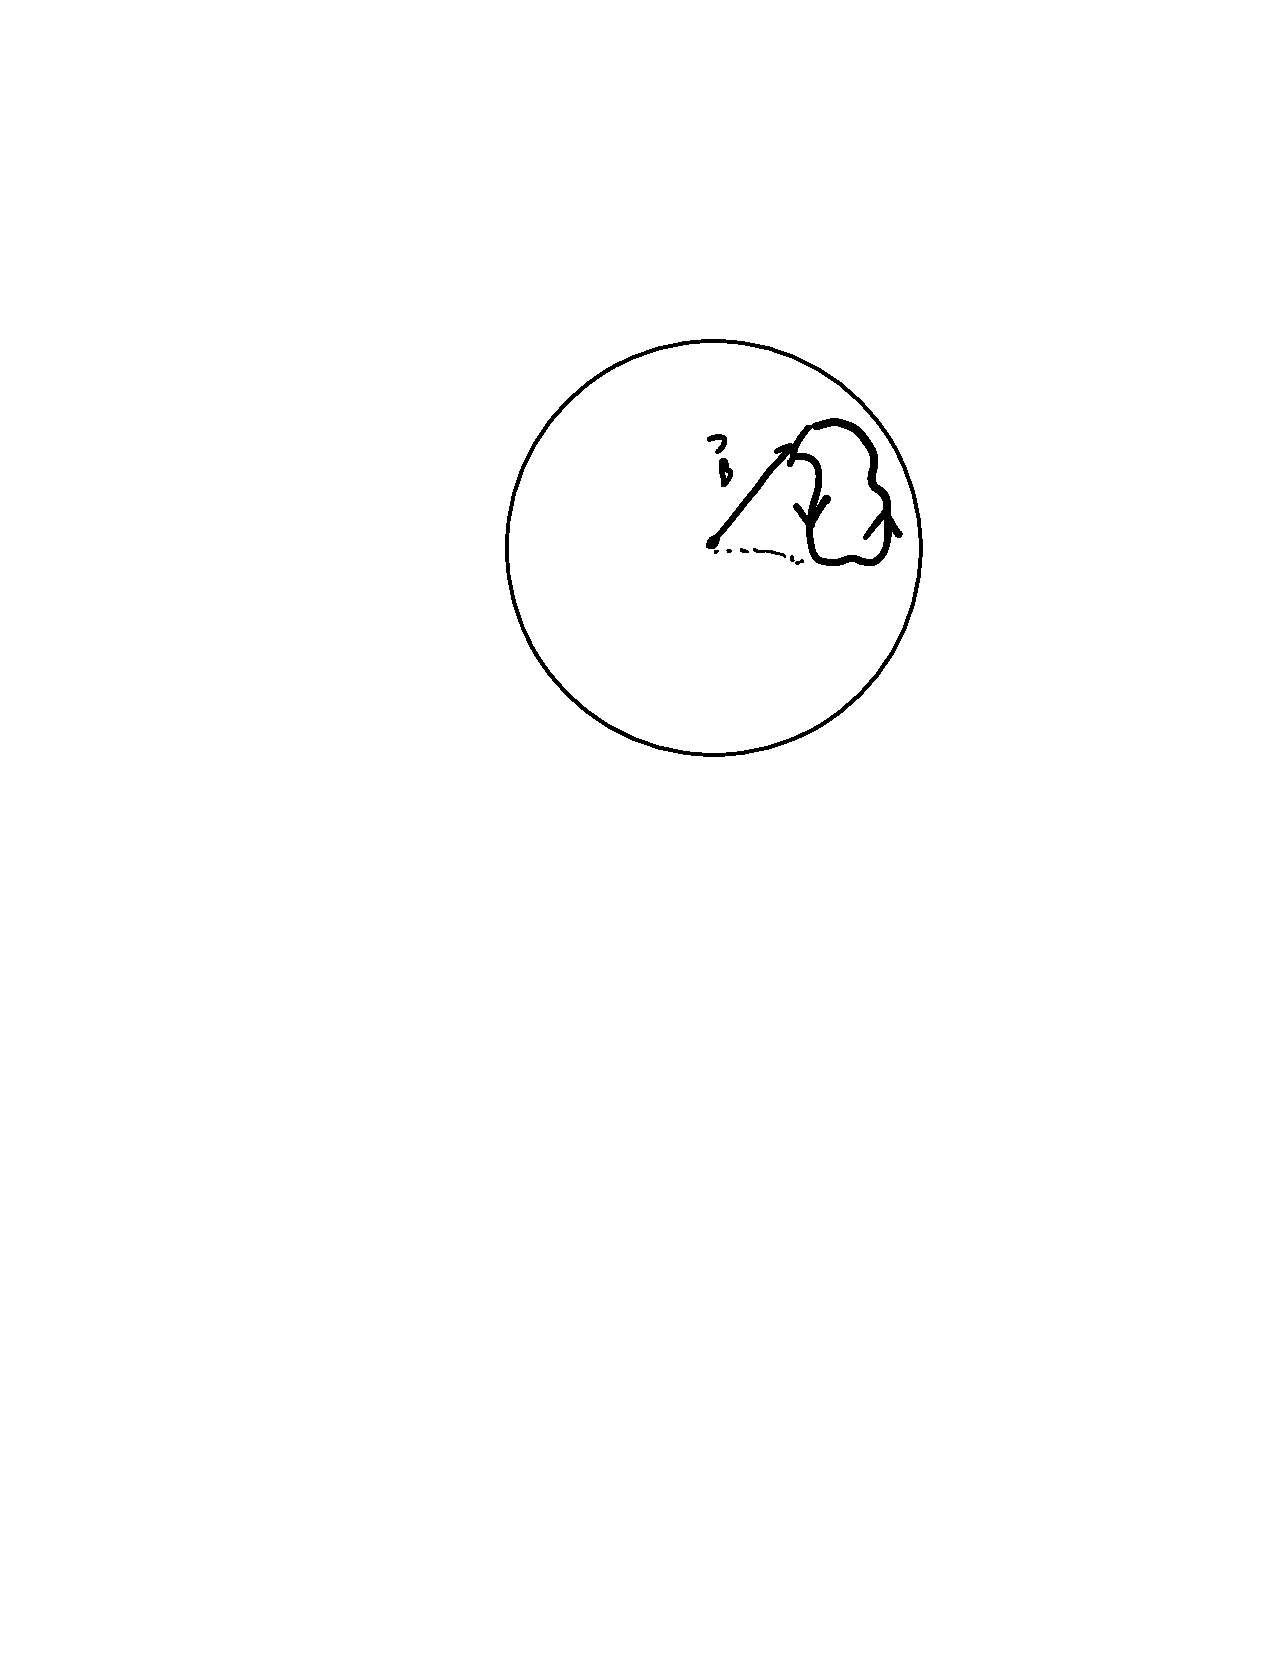
\includegraphics[scale=0.7]{Images/fig-sphereclosedcurve.pdf}

    \caption{We wish to calculate Berry's phase for a magnetic field $\v{B}$ that sweeps out an arbitrary closed curve on a sphere.}
    \label{fig-sphereclosedcurve}
\end{figure}

To this end consider the spinor corresponding to a spin pointing in the direction of $\v{B}(t)$:
\begin{equation}
    \chi_+ = \m{\cos(\frac{\theta(t)}{2}){t} \\ e^{i\phi(t)}\sin(\frac{\theta(t)}{2})}.
\end{equation}
with $\theta(t), \phi(t)$ the polar and azimuthal angles at time $t$. 

We wish to calculate the vector potential $\v{A}$ corresponding to $\v{B}$. To thid end, consider the gradient of $\chi_+$ in polar coordinates:
\begin{equation}
    \nabla \chi_+ = \rhat \dpd{}{r}\chi_+ + \frac{\thetahat}{r}\dpd{}{\theta}\chi_+ + \frac{\phihat}{r\sin\theta}\dpd{}{\phi}\chi_+ = \frac{1}{r}\left[\thetahat\m{-\frac{1}{2}\sin(\frac{\theta}{2}) \\ \frac{1}{2}e^{i\phi}\cos(\frac{\theta}{2})} + \frac{\phihat}{\sin\theta}\m{0 \\ e^{i\phi}\sin(\frac{\theta}{2})}\right]
\end{equation}
and so:
\begin{equation}
    \braket{\chi_+}{\nabla \chi_+} = \frac{1}{r}\thetahat\left[-\frac{1}{2}\sin(\frac{\theta}{2})\cos(\frac{\theta}{2}) + \frac{1}{2}\sin(\frac{\theta}{2})\cos(\frac{\theta}{2})\right] + i\frac{\phihat}{r\sin\theta}\sin^2(\frac{\theta}{2}) = i\frac{\phihat}{r\sin\theta}\sin^2(\frac{\theta}{2})
\end{equation}
and so:
\begin{equation}
    \v{A} = i\braket{\chi_+}{\nabla \chi_+} = -\phihat\frac{\sin^2(\frac{\theta}{2})}{r\sin\theta}
\end{equation}
Therefore recalling the Berry's phase as:
\begin{equation}
    \gamma = \oint \v{A} \cdot d\v{R} = \int \v{B} \cdot d\v{a}
\end{equation}
and calculating the magnetic field:
\begin{equation}
    \v{B} = \nabla \times \v{A} = \rhat \frac{1}{r\sin\theta}\dpd{}{\theta}\left(\sin\theta A_\phi\right) = -\frac{\rhat}{r^2}\frac{2\sin\frac{\theta}{2}\cos\frac{\theta}{2}}{\sin\theta}\frac{1}{2} = -\frac{\rhat}{r^2}\frac{1}{2}
\end{equation}
Which is the B-field of a magnetic monopole. Therefore computing Berry's phase:
\begin{equation}
    \gamma(T) = \int \v{B} \cdot d\v{a} = \int - \frac{1}{2r^2}r^2 d\Omega = -\frac{1}{2}\Omega
\end{equation}
where $\Omega$ is the solid angle subtended at the origin. We note that this is consistent with our example of the precessing $\v{B}$-field from last class. We also note again that this result is not dependent at all on the speed at which we move through configuration space.

\subsection{Gauge Potentials in QM}
In quantum mechanics (unlike in classical electromagnetism), Gauge potentials are physical. As a quick recap, the Hamiltonian with magnetic field was given by:
\begin{equation}
    H = \frac{(\v{p} - \frac{e}{c}\v{A})^2}{2m}
\end{equation} 
where $\v{A}$ is the Gauge potential. Under the Gauge transformation:
\begin{equation}
    \v{A}' = \v{A} + \nabla \Lambda
\end{equation}
the effect on the wavefunction is to induce a phase factor:
\begin{equation}
    \psi' = e^{i\frac{e}{\hbar c}\Lambda}\psi
\end{equation}

A clear demonstration of the physical effect of the Gauge potential is the Aharonov-Bohm effect. Consider a solenoid of radius $a$, and we place an charge $q$ on a bead of radius $R$ that goes around the solenoid.

\begin{figure}[htbp]
    \centering
    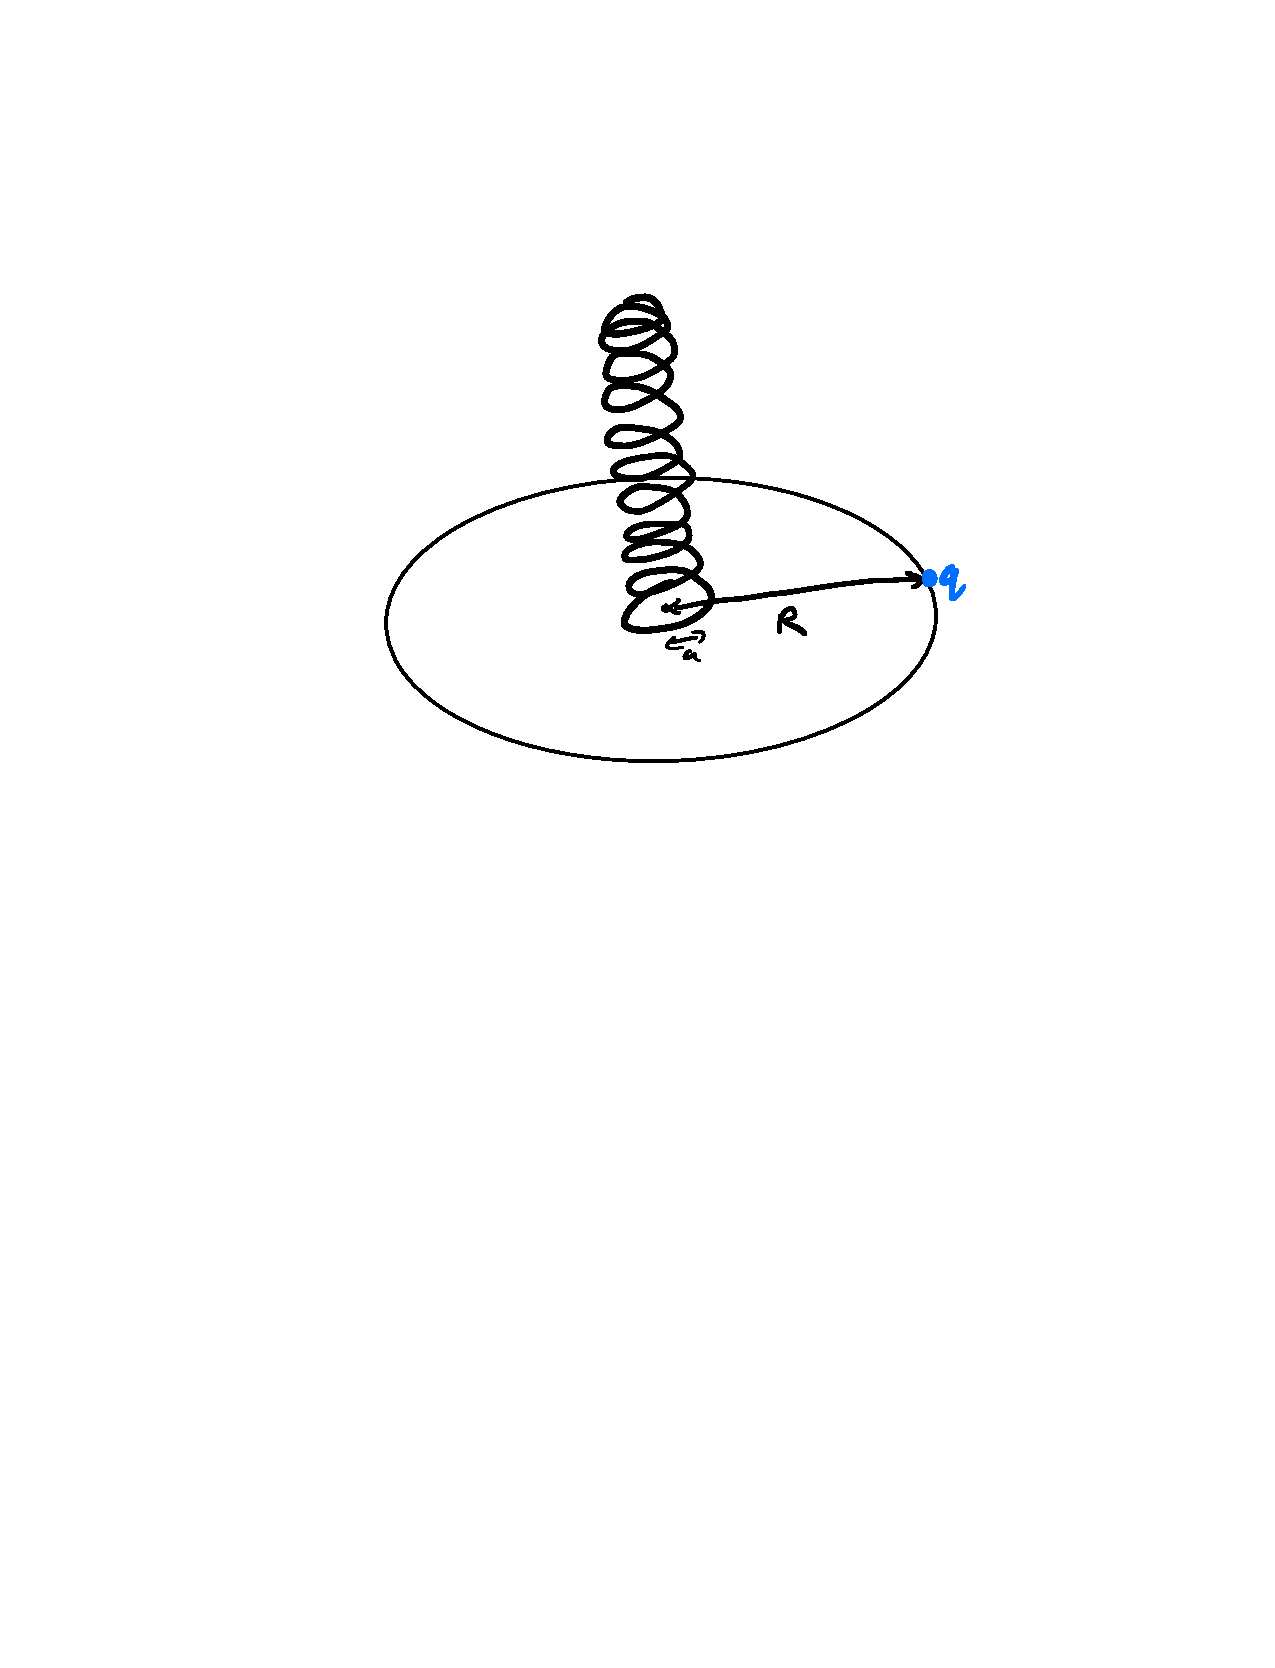
\includegraphics[scale=0.6]{Images/fig-solenoid.pdf}
    \caption{Setting of the Aharonov-Bohm effect - we consider a solenoid of radius $a$ and a loop of radius $R$ on which sits a charge $q$. The solenoid extends in the $\pm \zhat$ directions.}
    \label{fig-solenoid}
\end{figure}

The flux through the loop is $\Phi = \pi a^2 B$. For $r > a$, the Gauge potential is:
\begin{equation}
    A_\phi = \frac{\Phi}{2\pi}\frac{1}{r}\phihat, A_r = 0
\end{equation}
and so the magnetic field is:
\begin{equation}
    \v{B} = \nabla \times \v{A}
\end{equation}
of which the $z$-component is:
\begin{equation}
    B_z = \frac{1}{r}\left(\dpd{}{r}(rA_\phi) - \dpd{A_r}{\phi}\right) = 0
\end{equation}
so for $r > a$, $\v{B} = 0$. For $r \leq a$, we have:
\begin{equation}
    A_\phi = \frac{B\pi r^2}{2\pi a} = \frac{r}{2}B\phihat, \quad B_z = \frac{1}{r}\left(\dpd{}{r}(r^2 B)\right) = B
\end{equation} 

Returning back to $r > a$, we write:
\begin{equation}
    A_\phi = \frac{\Phi}{2\pi}\frac{1}{r}\phihat = \frac{\Phi}{r}\dpd{}{\phi}\left(\frac{\phi}{2\pi}\right)
\end{equation}
From here on I totally lose the thread of what's going on, so the notes become less coherent. When are we allowed to say:
\begin{equation}
    \v{A} = \nabla \Lambda
\end{equation}
and hence under the Gauge transformation $\v{A}' = 0$? The wavefunction is constrained to a single value. Let us write out the Hamiltonian:
\begin{equation}
    H = \frac{1}{2m}\left(\v{p} - \frac{e}{c}\v{A}\right)^2 = \frac{1}{2m}\left(-\frac{i\hbar}{R}\dpd{}{\phi} - \frac{e}{c}\frac{\Phi}{2\pi}\frac{1}{R}\right)^2 = \left(-\frac{i\hbar}{R}il - \frac{e\Phi}{2\pi c}\frac{1}{R}\right)
\end{equation}
If we find the eigenvalues and eigenstates:
\begin{equation}
    E = \frac{\hbar^2}{2mR^2}\left(l - \frac{e\Phi}{2\pi\hbar c}\right)^2
\end{equation}
which is very very stange; even though the particle is in a region where the fields are zero, nevertheless the spectrum is affected!

If $\frac{e\Phi}{2\pi \hbar c} = n \in ZZ$, we can write teh above as:
\begin{equation}
    E = \frac{\hbar^2}{2mR^2}(l - n)^2
\end{equation}
if this condition is not satisfied, we cannot do a gauge transformation - we are not always allowed to gauge transform in QM! (If we assume that we can do this Gauge transformation, then $H = \frac{p^2}{2m}$ with $p_\phi = \frac{i\hbar}{R}\dpd{}{\phi} = \frac{l\phi}{R}$ and $H = \frac{2mR^2}l\phi^2$ so $E = \frac{l}{2mR^2}$ for $l = 0, 1$). The wavefunctions transform as:
\begin{equation}
    \psi' = e^{i\frac{e}{\hbar c}\Lambda} = e^{i\frac{e}{\hbar c}\left(\frac{\Phi}{2\pi}\right)}.
\end{equation}  

Notably - the phase difference manifests itself in the spectrum, and is observable

